% Figures
\begin{figure*}[t]
    \centering
    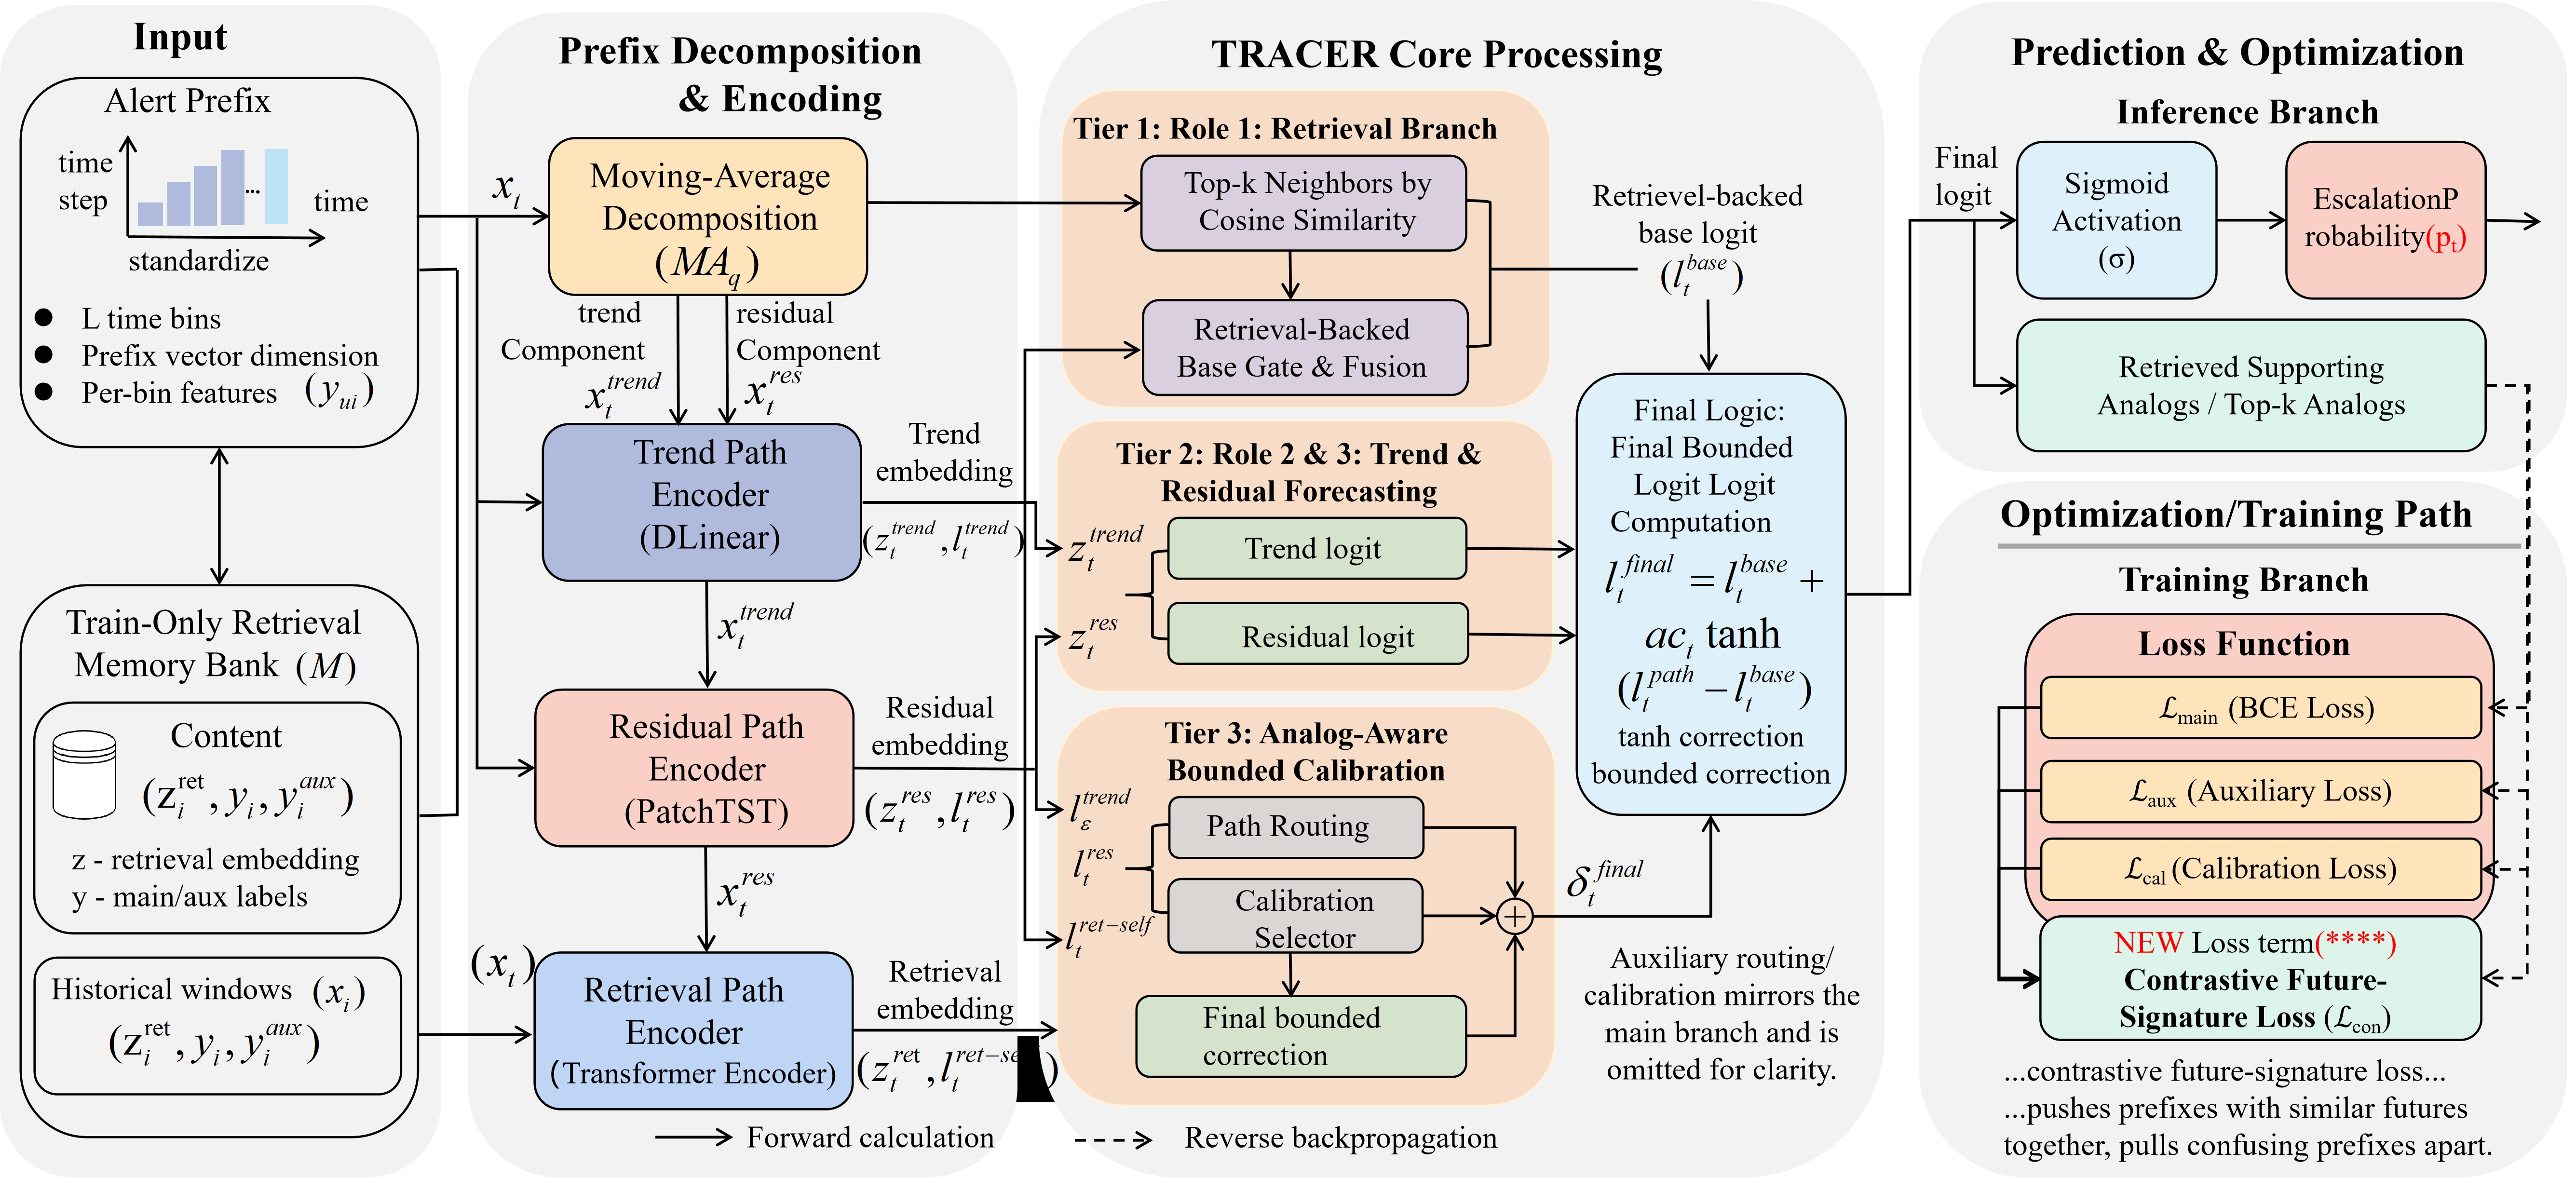
\includegraphics[width=\textwidth]{figures/f1_overview.png}
    \caption{Updated overview of the TRACER pipeline. An alert prefix is decomposed into slow trend and burst-sensitive residual views, while a train-only retrieval path queries historical analogs. The core first forms a retrieval-backed base score, then combines trend/residual forecasting, route selection, and bounded calibration to produce the final warning. The lower branch summarizes the training path with auxiliary-horizon, calibration, and future-signature contrastive objectives.}
    \label{fig:tracer-overview}
\end{figure*}

\begin{figure*}[t]
    \centering
    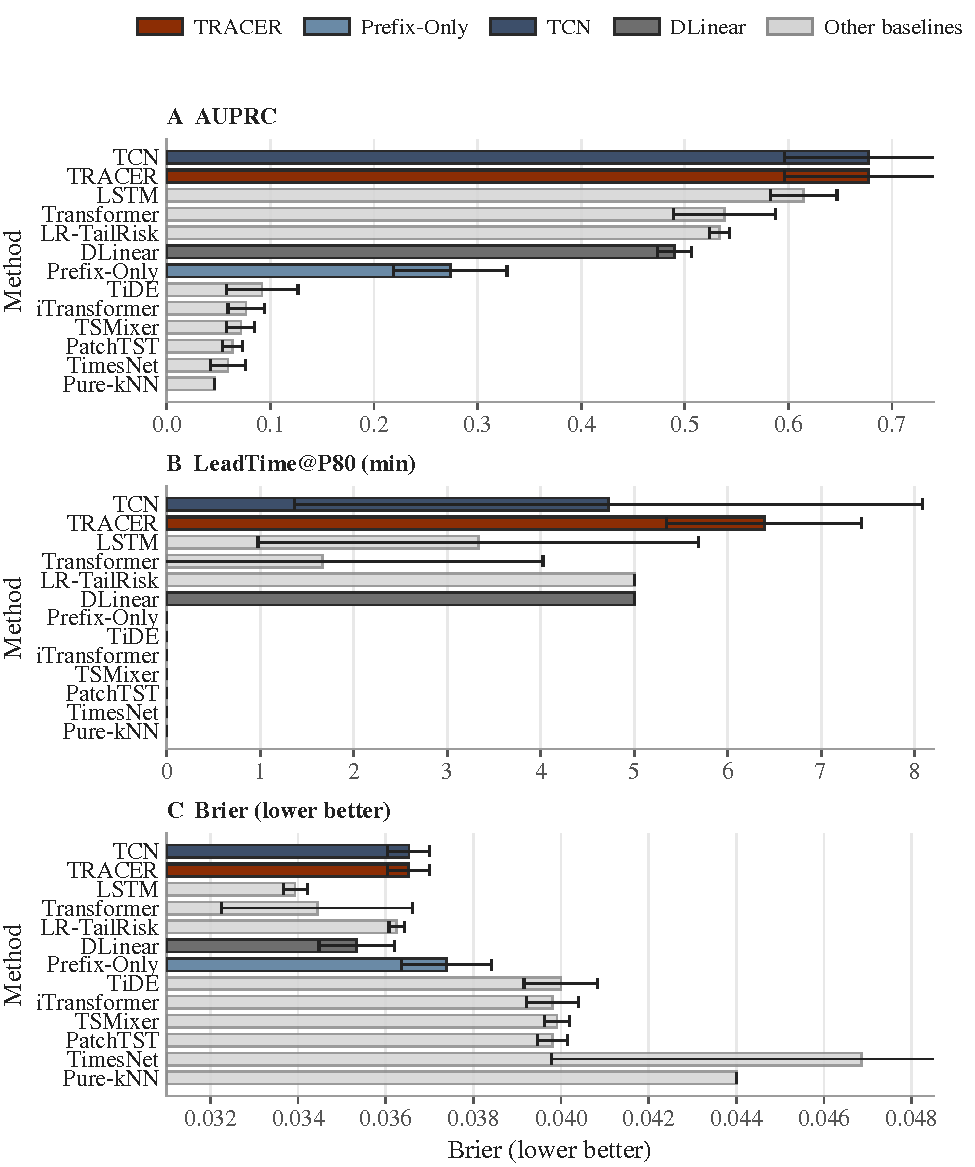
\includegraphics[width=\textwidth]{figures/fig_public_main_comparison.pdf}
    \caption{Chronological comparison on the public ATLASv2 benchmark.}
    \label{fig:public-main-comparison}
\end{figure*}

\begin{figure*}[t]
    \centering
    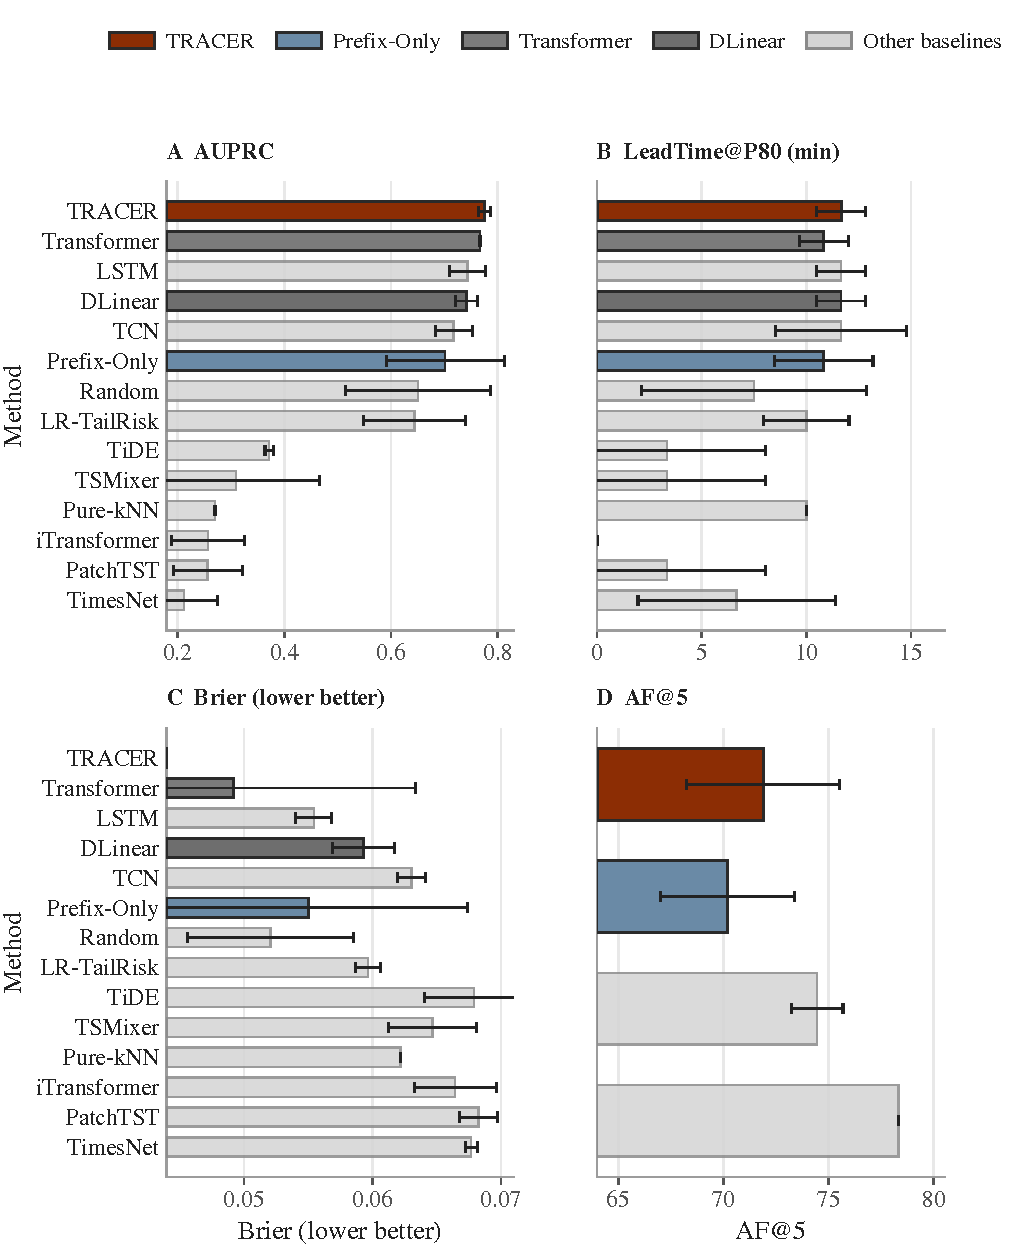
\includegraphics[width=\textwidth]{figures/fig_public_event_disjoint.pdf}
    \caption{Family-held-out event-disjoint comparison on the public ATLASv2 benchmark.}
    \label{fig:public-event-disjoint}
\end{figure*}

\begin{figure*}[t]
    \centering
    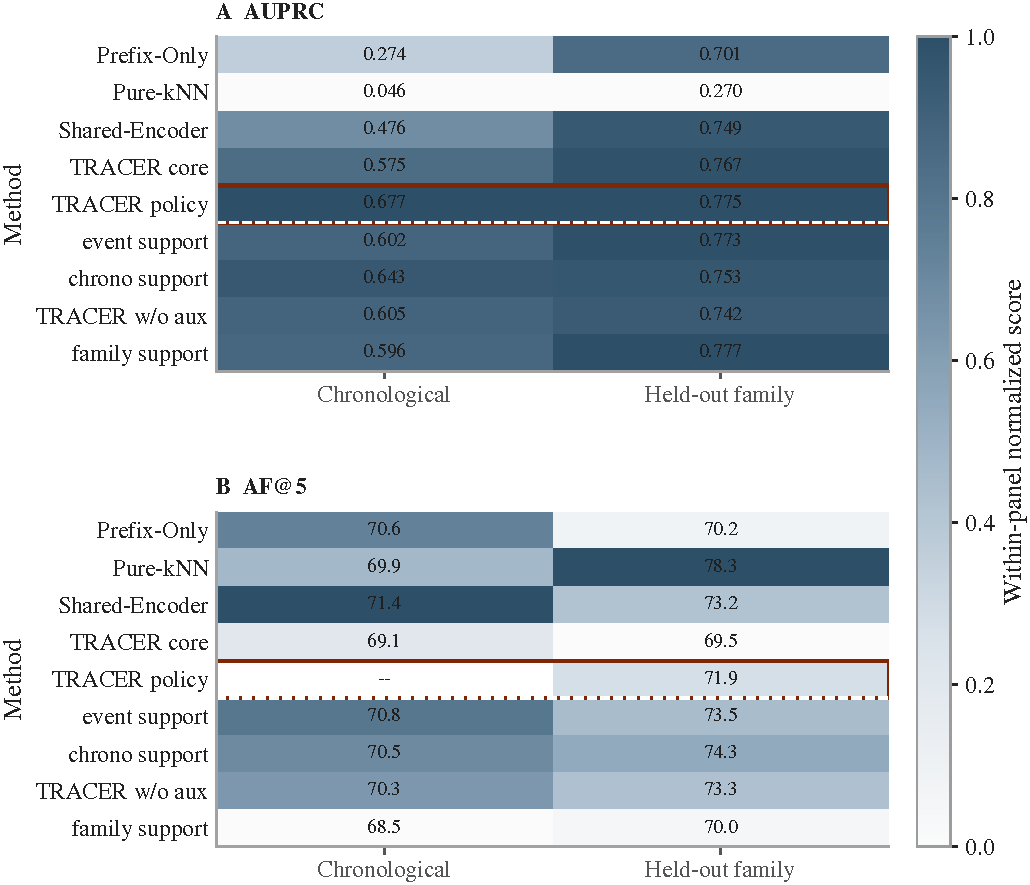
\includegraphics[width=\textwidth]{figures/fig_public_ablations.pdf}
    \caption{Novelty-isolation and ablation analysis on the public ATLASv2 benchmark.}
    \label{fig:public-ablations}
\end{figure*}

\begin{figure*}[t]
    \centering
    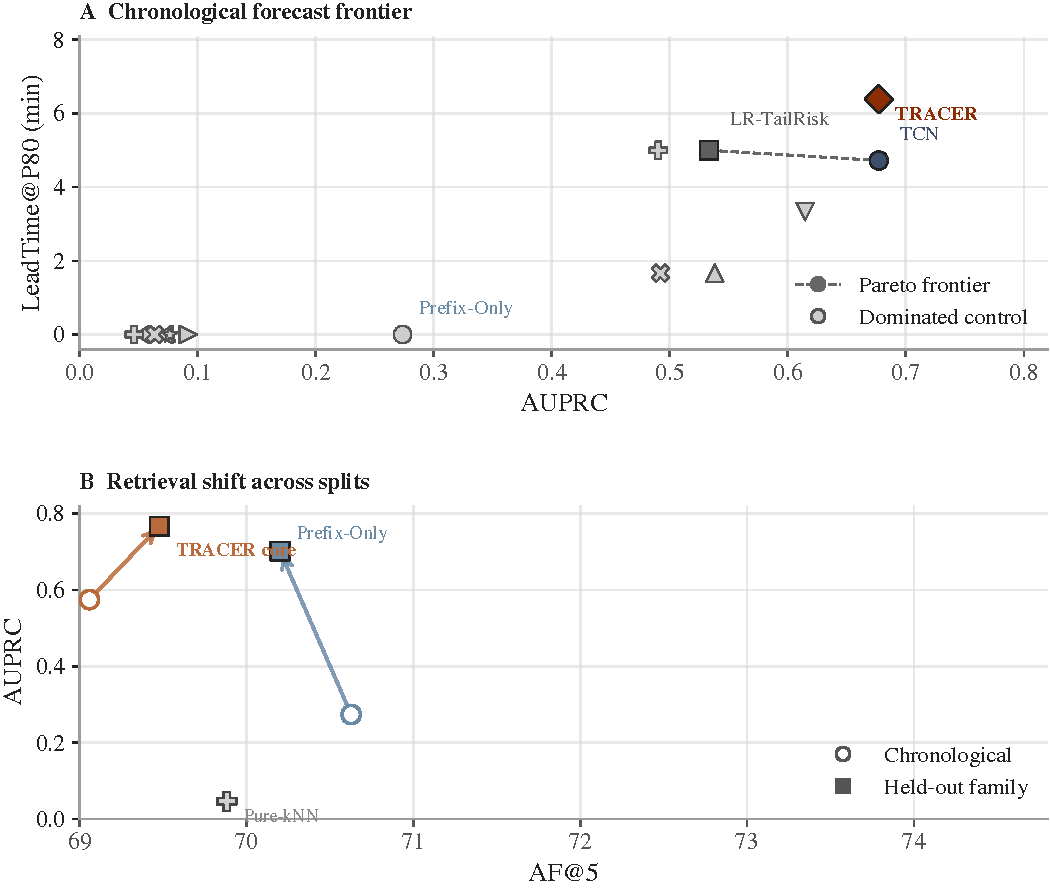
\includegraphics[width=\textwidth]{figures/fig_public_tradeoff_frontier.pdf}
    \caption{Trade-offs between forecasting accuracy, lead time, and analog quality on the public benchmark.}
    \label{fig:public-tradeoff-frontier}
\end{figure*}

\begin{figure*}[t]
    \centering
    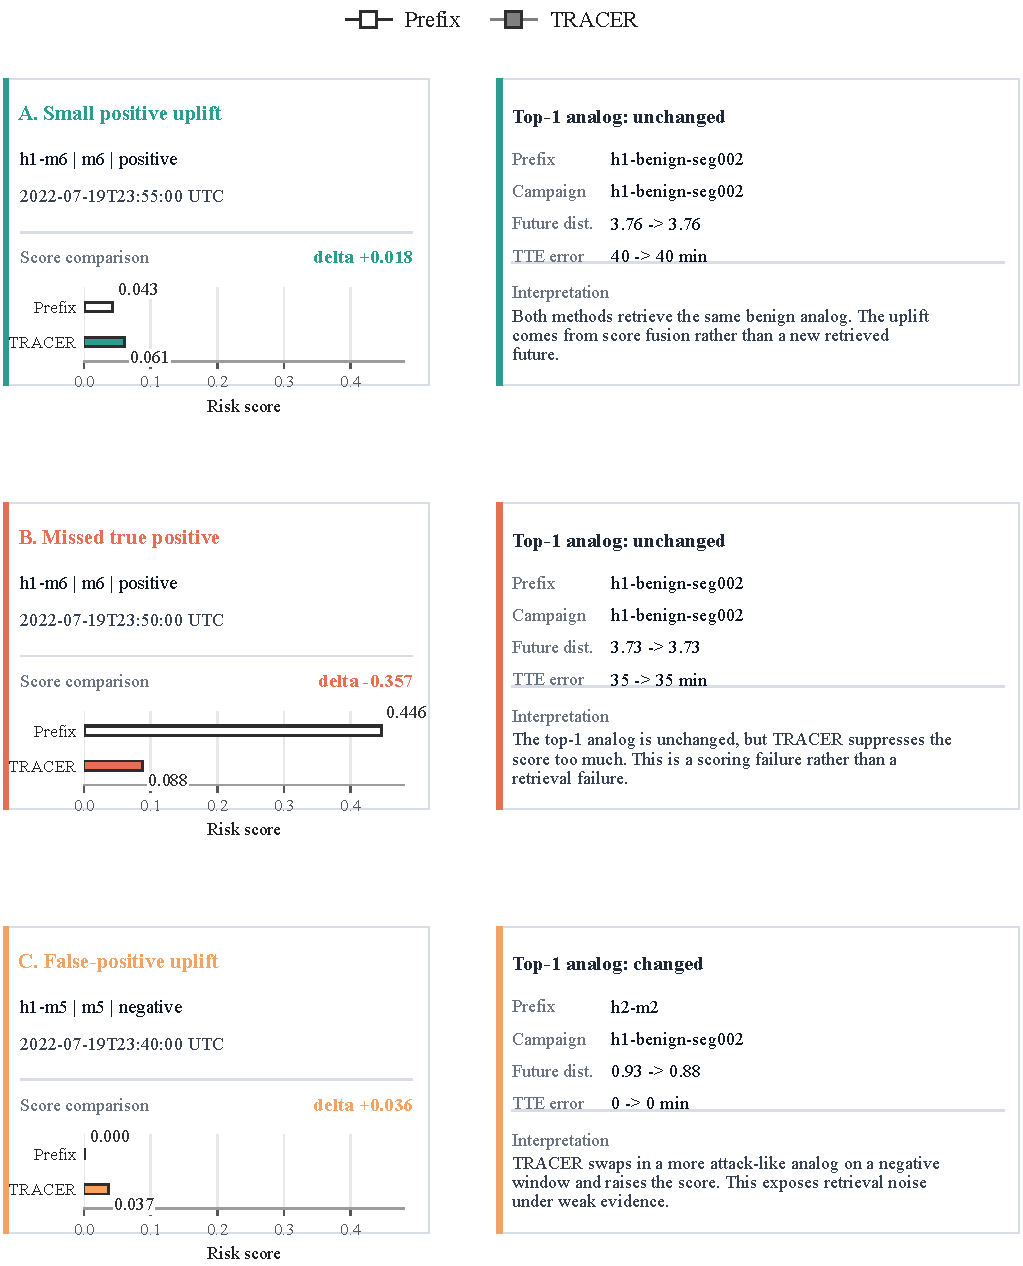
\includegraphics[width=\textwidth]{figures/fig_public_qualitative_cases.pdf}
    \caption{Qualitative diagnosis of retrieval behavior on the public ATLASv2 benchmark. The figure is intentionally limitation-oriented: the positive case is rare, and several cases share the same top-1 analog across methods.}
    \label{fig:public-qualitative-cases}
\end{figure*}

% Tables
\begin{table}[t]
\centering
\small
\setlength{\tabcolsep}{3.8pt}
\caption{Primary public ATLASv2 benchmark statistics. The held-out family set for the event-disjoint split is \texttt{atlasv2/s4}.}
\label{tab:atlasv2-public-stats}
\begin{tabular}{lccccc}
\toprule
Split & Windows & Positives & Pos.\ rate & Incidents & Families \\
\midrule
Train & 438 & 12 & 2.74\% & 24 & 23 \\
Dev & 155 & 4 & 2.58\% & 10 & 8 \\
Test & 170 & 7 & 4.12\% & 10 & 8 \\
Event-disjoint & 83 & 6 & 7.23\% & 6 & 6 \\
\bottomrule
\end{tabular}
\end{table}

\begin{table*}[t]
\centering
\small
\setlength{\tabcolsep}{3.5pt}
\caption{Public ATLASv2 benchmark results on chronological and family-held-out evaluation. Mean and standard deviation are computed over seeds 7, 13, and 21. Best available value in each metric column is bolded and the second-best value is underlined; lower is better for Brier and TTE-Err@1.}
\label{tab:atlasv2-public-main}
\maxtablewidth{
\begin{tabular}{llccccc}
\toprule
Split & Method & AUPRC & LeadTime@P80 & AF@5 & TTE-Err@1 & Brier \\
\midrule
Chronological & LR-TailRisk & $0.533 \pm 0.010$ & $\underline{5.00 \pm 0.00}$ & -- & -- & $0.036 \pm 0.000$ \\
Chronological & DLinear-Forecaster & $0.490 \pm 0.017$ & $\underline{5.00 \pm 0.00}$ & -- & -- & $\underline{0.035 \pm 0.001}$ \\
Chronological & TimesNet-Forecaster & $0.059 \pm 0.017$ & $0.00 \pm 0.00$ & -- & -- & $0.047 \pm 0.007$ \\
Chronological & TiDE-Forecaster & $0.092 \pm 0.035$ & $0.00 \pm 0.00$ & -- & -- & $0.040 \pm 0.001$ \\
Chronological & TSMixer-Forecaster & $0.072 \pm 0.013$ & $0.00 \pm 0.00$ & -- & -- & $0.040 \pm 0.000$ \\
Chronological & TCN-Forecaster & $\mathbf{0.677 \pm 0.081}$ & $4.72 \pm 3.36$ & -- & -- & $0.037 \pm 0.000$ \\
Chronological & LSTM-Forecaster & $\underline{0.615 \pm 0.032}$ & $3.33 \pm 2.36$ & -- & -- & $\mathbf{0.034 \pm 0.000}$ \\
Chronological & PatchTST-Forecaster & $0.064 \pm 0.010$ & $0.00 \pm 0.00$ & -- & -- & $0.040 \pm 0.000$ \\
Chronological & Small-Transformer-Forecaster & $0.538 \pm 0.049$ & $1.67 \pm 2.36$ & -- & -- & $\mathbf{0.034 \pm 0.002}$ \\
Chronological & iTransformer-Forecaster & $0.077 \pm 0.017$ & $0.00 \pm 0.00$ & -- & -- & $0.040 \pm 0.001$ \\
Chronological & Pure-kNN-Retrieval & $0.046 \pm 0.000$ & $0.00 \pm 0.00$ & $\underline{69.88 \pm 0.00}$ & $\mathbf{29.29 \pm 0.00}$ & $0.044 \pm 0.000$ \\
Chronological & Prefix-Only-Retrieval + Fusion & $0.274 \pm 0.055$ & $0.00 \pm 0.00$ & $\mathbf{70.63 \pm 1.25}$ & $\underline{29.76 \pm 2.36}$ & $0.037 \pm 0.001$ \\
Chronological & TRACER & $\mathbf{0.677 \pm 0.081}$ & $\mathbf{6.39 \pm 1.04}$ & -- & -- & $0.037 \pm 0.000$ \\
\midrule
Event-disjoint & DLinear-Forecaster & $0.742 \pm 0.021$ & $\mathbf{11.67 \pm 1.18}$ & -- & -- & $0.059 \pm 0.002$ \\
Event-disjoint & TimesNet-Forecaster & $0.213 \pm 0.062$ & $6.67 \pm 4.71$ & -- & -- & $0.068 \pm 0.000$ \\
Event-disjoint & TiDE-Forecaster & $0.372 \pm 0.008$ & $3.33 \pm 4.71$ & -- & -- & $0.068 \pm 0.004$ \\
Event-disjoint & TSMixer-Forecaster & $0.310 \pm 0.155$ & $3.33 \pm 4.71$ & -- & -- & $0.065 \pm 0.003$ \\
Event-disjoint & TCN-Forecaster & $0.717 \pm 0.035$ & $\mathbf{11.67 \pm 3.12}$ & -- & -- & $0.063 \pm 0.001$ \\
Event-disjoint & LSTM-Forecaster & $0.743 \pm 0.034$ & $\mathbf{11.67 \pm 1.18}$ & -- & -- & $0.055 \pm 0.001$ \\
Event-disjoint & PatchTST-Forecaster & $0.257 \pm 0.065$ & $3.33 \pm 4.71$ & -- & -- & $0.068 \pm 0.001$ \\
Event-disjoint & Small-Transformer-Forecaster & $\underline{0.767 \pm 0.000}$ & $\underline{10.83 \pm 1.18}$ & -- & -- & $\underline{0.049 \pm 0.014}$ \\
Event-disjoint & iTransformer-Forecaster & $0.258 \pm 0.069$ & $0.00 \pm 0.00$ & -- & -- & $0.066 \pm 0.003$ \\
Event-disjoint & Prefix-Only-Retrieval + Fusion & $0.701 \pm 0.110$ & $\underline{10.83 \pm 2.36}$ & $\underline{70.20 \pm 3.20}$ & $\underline{26.94 \pm 4.32}$ & $0.055 \pm 0.012$ \\
Event-disjoint & TRACER & $\mathbf{0.775 \pm 0.012}$ & $\mathbf{11.67 \pm 1.18}$ & $\mathbf{71.89 \pm 3.63}$ & $\mathbf{25.28 \pm 1.57}$ & $\mathbf{0.035 \pm 0.002}$ \\
\bottomrule
\end{tabular}
}
\end{table*}

\begin{table*}[t]
\centering
\small
\setlength{\tabcolsep}{3.5pt}
\caption{Public ATLASv2 chronological operating-point comparison for TRACER and related support variants. Mean and standard deviation are computed over seeds 7, 13, and 21 when available. Best available value in each metric column is bolded and the second-best value is underlined; lower is better for Brier and TTE-Err@1.}
\label{tab:atlasv2-public-ablations}
\maxtablewidth{
\begin{tabular}{lccccc}
\toprule
Method & AUPRC & LeadTime@P80 & AF@5 & TTE-Err@1 & Brier \\
\midrule
No-Memory Forecaster & $0.538 \pm 0.049$ & $1.67 \pm 2.36$ & -- & -- & $0.034 \pm 0.002$ \\
Pure-kNN-Retrieval & $0.046 \pm 0.000$ & $0.00 \pm 0.00$ & $69.88 \pm 0.00$ & $29.29 \pm 0.00$ & $0.044 \pm 0.000$ \\
Prefix-Only-Retrieval + Fusion & $0.274 \pm 0.055$ & $0.00 \pm 0.00$ & $70.63 \pm 1.25$ & $29.76 \pm 2.36$ & $0.037 \pm 0.001$ \\
Shared-Encoder TRACER & $0.476 \pm 0.068$ & $4.17 \pm 3.12$ & $\mathbf{71.41 \pm 0.35}$ & $29.05 \pm 2.05$ & $0.036 \pm 0.002$ \\
TRACER Core Mode & $0.575 \pm 0.065$ & $3.33 \pm 2.36$ & $69.06 \pm 1.08$ & $27.38 \pm 1.35$ & $\mathbf{0.029 \pm 0.002}$ \\
TRACER (adaptive policy) & $\mathbf{0.677 \pm 0.081}$ & $\underline{6.39 \pm 1.04}$ & -- & -- & $0.037 \pm 0.000$ \\
Event-Focused TRACER Variant & $0.602 \pm 0.053$ & $4.17 \pm 3.12$ & $\underline{70.78 \pm 1.69}$ & $\underline{27.14 \pm 3.25}$ & $\underline{0.033 \pm 0.001}$ \\
Chronology Support Line & $\underline{0.643 \pm 0.051}$ & $\mathbf{7.50 \pm 2.04}$ & $70.51 \pm 1.53$ & $27.38 \pm 1.35$ & $0.034 \pm 0.001$ \\
TRACER w/o auxiliary horizon & $0.605 \pm 0.023$ & $4.17 \pm 3.12$ & $70.31 \pm 0.62$ & $28.10 \pm 2.36$ & $0.034 \pm 0.001$ \\
Held-Out-Family Support Line & $0.596 \pm 0.062$ & $5.83 \pm 1.18$ & $68.47 \pm 1.36$ & $\mathbf{26.43 \pm 0.00}$ & $0.035 \pm 0.000$ \\
\bottomrule
\end{tabular}
}
\end{table*}

\begin{table}[t]
\centering
\small
\setlength{\tabcolsep}{3.8pt}
\caption{Secondary workbook-derived public probe statistics. This split is chronological-only and is used as supplementary evidence.}
\label{tab:atlasv2-workbook-stats}
\begin{tabular}{lccccc}
\toprule
Split & Windows & Positives & Pos.\ rate & Incidents & Families \\
\midrule
Train & 1593 & 10 & 0.63\% & 8 & 6 \\
Dev & 520 & 0 & 0.00\% & 4 & 3 \\
Test & 519 & 13 & 2.50\% & 4 & 3 \\
\bottomrule
\end{tabular}
\end{table}

\begin{table*}[t]
\centering
\small
\setlength{\tabcolsep}{3.5pt}
\caption{Secondary workbook-derived public probe with expanded parametric and retrieval baselines. This table is supplementary because the workbook split is not family-held-out. Best available value in each metric column is bolded and the second-best value is underlined; lower is better for Brier and TTE-Err@1.}
\label{tab:atlasv2-public-robustness}
\maxtablewidth{
\begin{tabular}{lccccc}
\toprule
Method & AUPRC & LeadTime@P80 & AF@5 & TTE-Err@1 & Brier \\
\midrule
LR-TailRisk & $0.023 \pm 0.003$ & $0.00 \pm 0.00$ & -- & -- & $\underline{0.026 \pm 0.001}$ \\
TCN-Forecaster & $0.032 \pm 0.001$ & $0.00 \pm 0.00$ & -- & -- & $\mathbf{0.025 \pm 0.000}$ \\
LSTM-Forecaster & $\mathbf{0.232 \pm 0.143}$ & $0.00 \pm 0.00$ & -- & -- & $\mathbf{0.025 \pm 0.000}$ \\
Small-Transformer-Forecaster & $0.150 \pm 0.030$ & $\mathbf{3.33 \pm 2.36}$ & -- & -- & $\mathbf{0.025 \pm 0.000}$ \\
Prefix-Only-Retrieval + Fusion & $\underline{0.162 \pm 0.032}$ & $\underline{1.67 \pm 2.36}$ & $\mathbf{81.70 \pm 0.19}$ & $\mathbf{3578.1 \pm 779.7}$ & $\mathbf{0.025 \pm 0.000}$ \\
TRACER & $0.133 \pm 0.141$ & $0.00 \pm 0.00$ & -- & -- & $\mathbf{0.025 \pm 0.000}$ \\
Shared-Encoder TRACER & $0.070 \pm 0.026$ & $\underline{1.67 \pm 2.36}$ & $\underline{81.61 \pm 1.26}$ & $\underline{4403.2 \pm 144.3}$ & $\mathbf{0.025 \pm 0.000}$ \\
\bottomrule
\end{tabular}
}
\end{table*}


% Summary data: atlasv2_public_seed_summary.json, atlasv2_public_seed_summary.csv
